%%%%%%%%%%%%%%%%%%%%%%%%%%%%%%%%%%%%%%%%%%%%%%%%%%%%%%%%%%%%%%%%
% Sim
%%%%%%%%%%%%%%%%%%%%%%%%%%%%%%%%%%%%%%%%%%%%%%%%%%%%%%%%%%%%%%%%
\section{仿真}
本文使用基于C++的仿真器\cite{olzhn2021}进行仿真。
下文介绍各部分设计原理。

% ////////////////////////////////////////
\subsection{被控对象建模}
可以用上一节中推导出的式\eqref{eqModelTotal}建立被控对象微分方程,
若忽略火星自转的影响,
也可以建立向量形式的微分方程
\begin{equation}
    \ddot{\vec{r}} = \frac{\mu}{||\vec{r}||^3}\vec{r}+\vec{L}+\vec{D} \label{eqSimFA}
\end{equation}
其中阻力向量为
\begin{align}
    \vec{D} = -D\frac{\vec{v}}{||\vec{v}||} \label{eqSimFD}
\end{align}
升力向量$\vec{L}$与铅垂面夹角为倾侧角$\sigma$,
为了能将$\vec{L}$用其他已知向量表示,
需要构造一对与$\vec{L}$同平面的正交单位向量。
已知$\vec{v}$与$\vec{r}$张成铅垂面,
另构造一个垂直于铅垂面且在惯性系中方向向上的单位向量$\vec{n}_2$,
和另一个与$\vec{r}$同方向的单位向量$\vec{n}_1$,
则$\vec{n}_1$位于铅垂面内,
此时$\vec{L}$与$\vec{n}_1$的夹角即为倾侧角,
$\vec{n}_1$和$\vec{n}_2$即为用于表示$\vec{L}$的正交单位向量,
即
\begin{align}
    \vec{n}_2 =& \frac{\vec{r}\times\vec{v}}{||\vec{r}\times\vec{v}||} \notag\\
    \vec{L} =& \vec{n}_1\cos\sigma + \vec{n}_2\sin\sigma \label{eqSimFL}
\end{align}
% 在升力系数$C_L$和阻力系数$C_D$均为常数的假设下,
% 升力向量$\vec{L}$和阻力向量$\vec{D}$的夹角保持不变,
微分方程式\eqref{eqSimFA}\eqref{eqSimFD}\eqref{eqSimFL}共同组成被控对象模型。
建立飞行器被控对象模型的模块框图如图\ref{figSimPlant}所示。
\begin{center}
	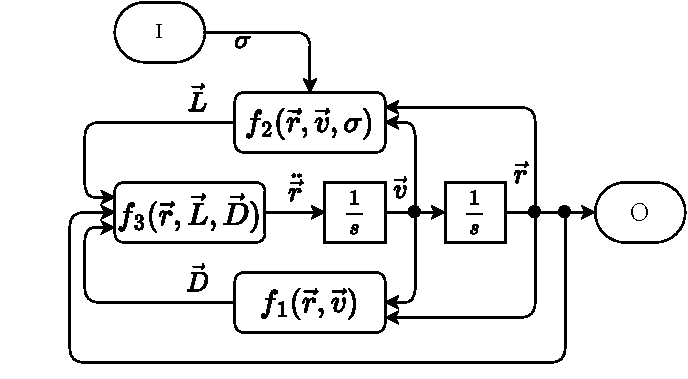
\includegraphics[scale=0.8]{plant.pdf}  \\
	\figcaption{被控对象模型的模块框图}\label{figSimPlant}
\end{center}
图中,被控对象的输入(控制量)为倾侧角$\sigma$,
输出为位置$\vec{r}$。
图中的两个多输入单输出函数分别为式\eqref{eqSimFLDTotal}\eqref{eqSimFATotal}
\begin{align}
    \left\{\begin{aligned}
    h =& ||\vec{r}||-R \\
    \rho =& \rho_0e^{-h/h_s} \\
    D =& \frac{1}{2}\rho||\vec{v}||^2S_{\text{ref}}C_D \\
    \vec{D} =& f_1(\vec{r},\vec{v}) = -D\frac{\vec{v}}{||\vec{v}||} \\
    L =& DC_{LD} \\
    \vec{n}_1 =& \frac{\vec{r}}{||\vec{r}||} \\
    \vec{n}_2 =& \frac{\vec{r}\times\vec{v}}{||\vec{r}\times\vec{v}||} \\
    \vec{L} =& f_2(\vec{r},\vec{v},\sigma) = L(\vec{n}_1\cos\sigma + \vec{n}_2\sin\sigma) \\
    \vec{f}_{LD} =& f_{LD}(\vec{r},\vec{v},\sigma) = \vec{L} + \vec{D}
\end{aligned}\right. \label{eqSimFLDTotal}
\end{align}
\begin{equation}
    \ddot{\vec{r}} = f_A(\vec{r},\vec{f}_{LD}) = \frac{\mu}{||\vec{r}||^3}\vec{r}+\frac{\vec{f}_{LD}}{m} \label{eqSimFATotal}
\end{equation}
式中$R$为火星半径,$C_{LD}=C_L/C_D$为升阻比。

% ////////////////////////////////////////
\subsection{仿真结果}
首先展示不使用制导律,控制量输出常值的仿真结果。
进入点轨道参数和控制量如下。
\begin{center}\begin{tabular}{ll}
    \toprule
    名称 & 值 \\
    \midrule
    进入速度(km/s) & 5.8 \\
    进入点高度(km) & 125 \\
    进入航迹角(rad) & 0.175(10$^\circ$) \\
    进入航向角(rad) & 0 \\
    倾侧角(rad) & 1 \\
    \bottomrule
\end{tabular}\end{center}

\begin{center}
	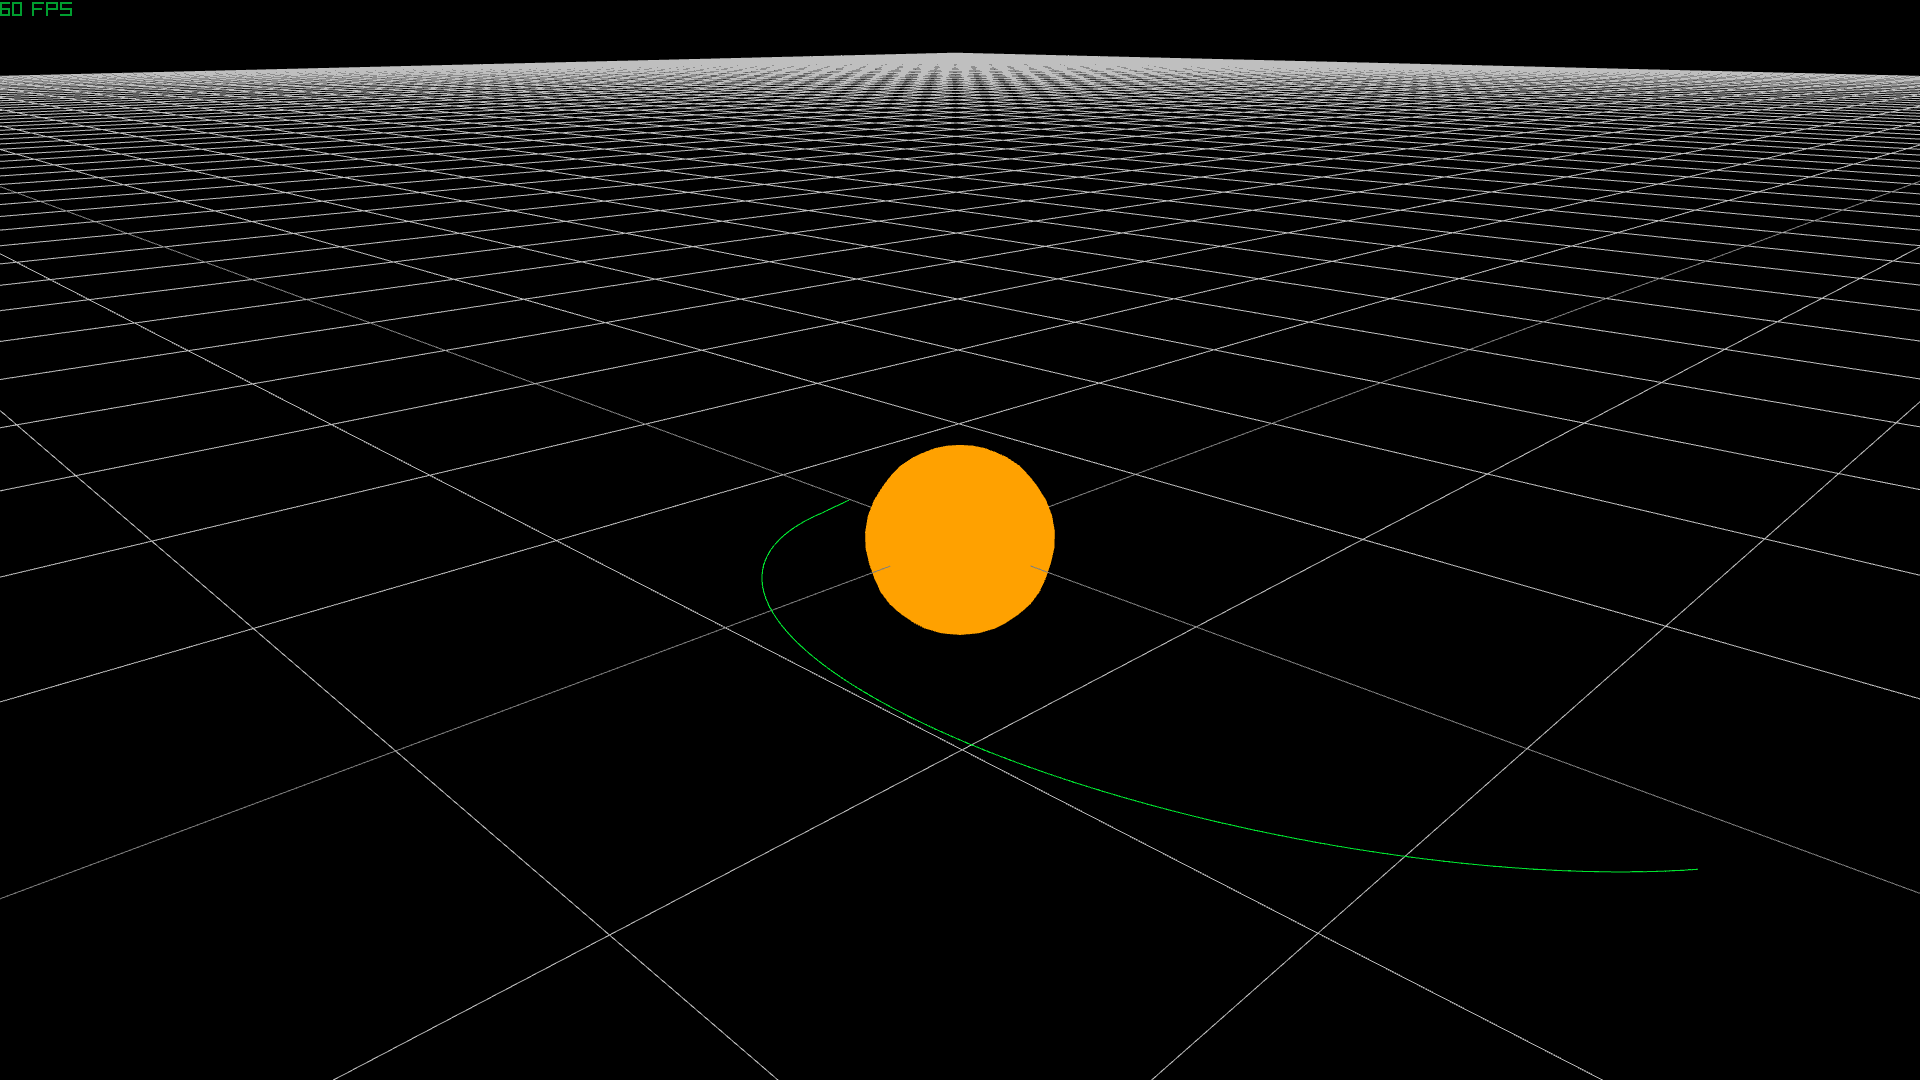
\includegraphics[scale=0.2]{sim1Verticalview.png}  \\
	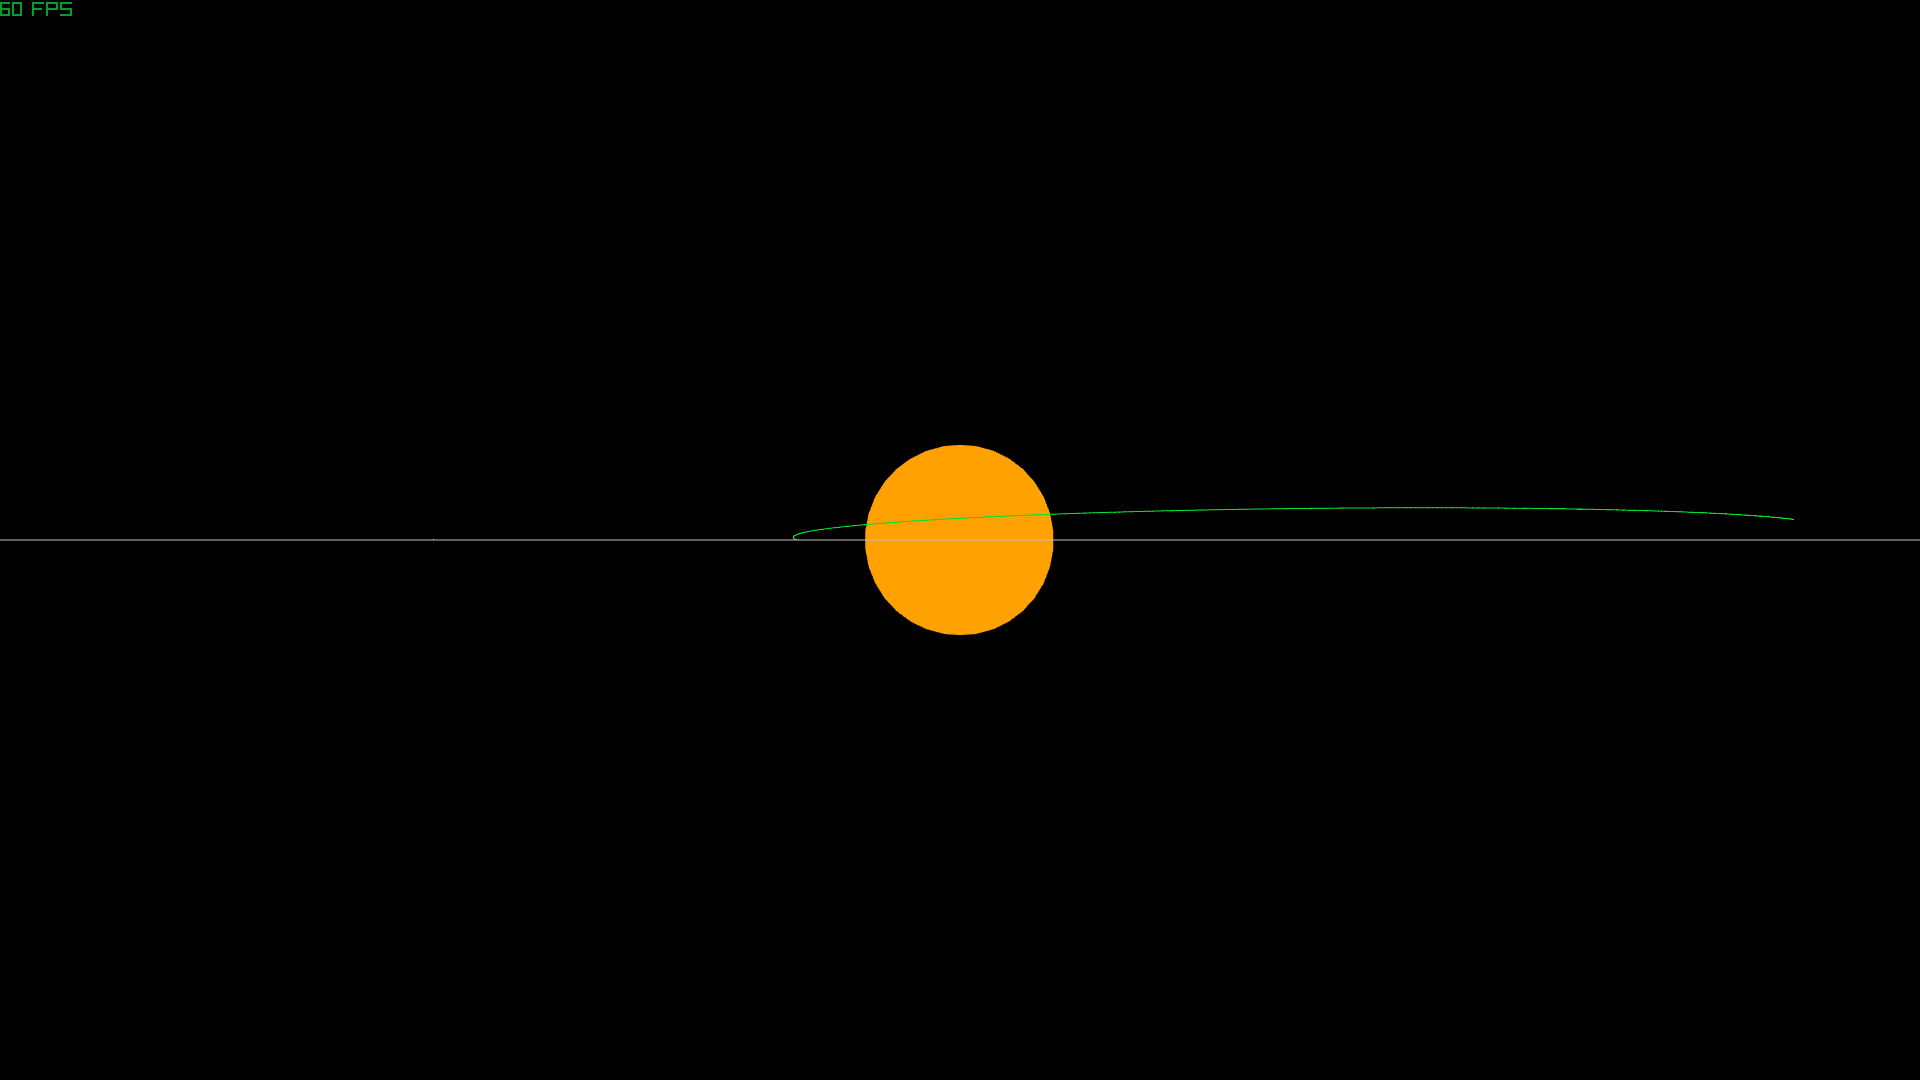
\includegraphics[scale=0.2]{sim1Sideview.png}  \\
	\figcaption{确定轨迹仿真结果}\label{figSim1}
\end{center}


